\documentclass[presentation]{beamer}
\usetheme{CambridgeUS}
\usecolortheme{orchid}

\definecolor{themeColor}{HTML}{4e6eff}

\setbeamercolor*{structure}{bg=black,fg=themeColor}

\setbeamercolor*{palette primary}{use=structure,fg=white,bg=structure.fg}
\setbeamercolor*{palette secondary}{use=structure,fg=white,bg=structure.fg!75}
\setbeamercolor*{palette tertiary}{use=structure,fg=white,bg=structure.fg!50!black}
\setbeamercolor*{palette quaternary}{fg=white,bg=black}

\setbeamercolor{section in toc}{fg=black,bg=white}
\setbeamercolor{alerted text}{use=structure,fg=structure.fg!50!black!80!black}

\setbeamercolor{titlelike}{parent=palette primary,fg=structure.fg!50!black}
\setbeamercolor{frametitle}{bg=structure.fg!10!white,fg=structure.fg!50!black!80!black}

\setbeamercolor*{titlelike}{parent=palette primary}


\usepackage[utf8]{inputenc}
\usepackage{amssymb}
\usepackage{graphicx}
\usepackage{subfigure}
\usepackage{multirow}
\usepackage{hhline}
\usepackage{amsfonts,amstext,amssymb,wasysym}
\usepackage{fancyvrb}
\usepackage{alltt}
\usepackage{textcomp}
\usepackage{url}
\usepackage{multimedia,pgf}
\usepackage{geometry}
\usepackage{minted}
\usepackage{bibentry}
% % \usepackage{framed}
\usepackage{cleveref}
\nobibliography*

\title[02 - Teamwork]{\small{\input{../coursetitle}} \\
\normalsize{Productive parallel teamwork: Decentralized Version Control Systems}}

% ! TeX root = 01-Introduction/01-Introduction.tex
\author[D. Pianini]{
Danilo Pianini\\
\texttt{{\footnotesize danilo.pianini@unibo.it}}}

\institute[UniBo]
{\textsc{Alma Mater Studiorum}---Universit\`a di Bologna}

\date[\today{}]{\input{../context} \\
\scriptsize \input{../date} - \input{../place} 
}

\pgfdeclareimage[height=0.625cm]{university-logo}{../images/logo}
\logo{\pgfuseimage{university-logo}}


\begin{document}

% ! TeX root = 01-Introduction/01-Introduction.tex
\AtBeginSubsection[]{%
  \begin{frame}<beamer>
    \frametitle{Outline}
    \tableofcontents[currentsection,currentsubsection]
  \end{frame}
  \addtocounter{framenumber}{-1}% If you don't want them to affect the slide number
}


\newcommand{\codefile}[3]{
	\begin{block}{\texttt{#1}}
		\inputminted[fontsize=#2,linenos=true,breaklines=true]{#3}{#1}
	\end{block}
}
%===============================================================================
\frame[label=coverpage]{\titlepage}
%===============================================================================

%===============================================================================
%===============================================================================
\section*{Outline}
%===============================================================================
%===============================================================================

\frame{\tableofcontents}

%===============================================================================
%===============================================================================

\section{Versioning}

\subsection{Motivation}

\begin{frame}{Keep track of changes}
    Have you ever had the need to:
    \begin{itemize}
        \item roll back some project to a working version
        \item roll back some subpart of a project to an older version
        \item compare with the previous state and see the changes
    \end{itemize}
    Many had
\end{frame}

\begin{frame}{Do it yourself}
    Basic strategy everybody applied at least once (be honest...)
    \begin{enumerate}
        \item work on project
        \item if status is kinda ok, copy everything in a folder
        \item optionally, put a version or a date to the folder name
        \item optionally, compress the folder
        \item go to 1
    \end{enumerate}
    \begin{block}{Why is bad}
        \begin{itemize}
            \item Expensive in time
            \item Snapshotting costs a lot in space (tons of duplication) 
            \item Difficult to compare with previous
            \item Very hard to roll back different parts at different versions
            \item Remembering differences between versions is impossible over time
        \end{itemize}
    \end{block}
\end{frame}

\begin{frame}{Let a tool do it}
    \begin{block}{Desiderata}
        \begin{itemize}
            \item Differential tracking: only store differences, not copies
            \item History navigation: ability to roll back in time
            \item Partial roll backs: ability to roll back only sub-part of the project
            \item Annotation of versions with messages
            \item Annotation of versions with numbers or names
            \item Automatic generation of dates
            \item Author tracking
            \item Possibility to select the parts of a project to save
            \begin{itemize}
                \item You are only interested in non-regenerable resources
                \item They often are only a part of a project
            \end{itemize}
        \end{itemize}
    \end{block}
\end{frame}

\subsection{git as versioning tool}

\begin{frame}[fragile]{Bits of history}
	\begin{itemize}
		\item In April 2005, BitKeeper, the SCM Linux was developed with, withdrawn the free (as in beer) use
		\item No other SCM met the requirements of Torvalds
		\begin{itemize}
			\item Performance was the \textit{real} issue with such a code base
		\end{itemize}
		\item Torvalds decided to write his own
		\item The project was successful, and Torvalds appointed maintenance to Hamano
	\end{itemize}
	\begin{block}{Why the name}
		\begin{quote}
			I'm an egotistical bastard, and I name all my projects after myself. First 'Linux', now 'git'. \footnote{\tiny{From the project Wiki. ``git'' is slang for ``pig headed, think they are always correct, argumentative''}}
			\begin{flushright}
				\normalfont{--- Linus Torvalds}
			\end{flushright}
		\end{quote}
	\end{block}
\end{frame}

\begin{frame}[fragile]{The \texttt{git} \texttt{README.md} file}
	\begin{block}{}
		\begin{minted}[fontsize=\footnotesize]{yaml}
GIT - the stupid content tracker

"git" can mean anything, depending on your mood.

 - random three-letter combination that is pronounceable, and not
   actually used by any common UNIX command.  The fact that it is a
   mispronounciation of "get" may or may not be relevant.
 - stupid. contemptible and despicable. simple. Take your pick from the
   dictionary of slang.
 - "global information tracker": you're in a good mood, and it actually
   works for you. Angels sing, and a light suddenly fills the room. 
 - "goddamn idiotic truckload of sh*t": when it breaks
		\end{minted}
	\end{block}
\end{frame}

\begin{frame}[fragile]{Features}
	\begin{itemize}
		\item UNIX-oriented: tracks stuff like UNIX file permits.
		\item Distributed development (the whole development history is copied locally)
		\item Diff-based history tracking
		\item Implicit file naming (history preserved on renames)
		\item Very strong support to non-linear development
		\item Written in C
		\item Approximately 10 times faster than Mercurial, 100 times faster than other DVCS (e.g. Bazaar)
		\item Uses existing protocols (ssh, http, ftp, rsync...)
		\item Pluggable merge strategies (defaults to recursive three-ways merge or octopus for 3+ heads)
	\end{itemize}
\end{frame}

\newcommand{\fullsizeimage}[1]{\includegraphics[width=\textwidth,height=.80\textheight,keepaspectratio]{#1}}

\begin{frame}[allowframebreaks]{Popularity (data from: \url{http://archive.is/bBNkZ})}
    \begin{center}
        \fullsizeimage{img/questions}
        \fullsizeimage{img/search}
        \fullsizeimage{img/questionsbynum}
        \fullsizeimage{img/questionsbyshare}
        \fullsizeimage{img/interest}
    \end{center}
\end{frame}

\subsection{Terminology and basic concepts}

\begin{frame}{Repository}
    Folder containing all the files tracked by git. Includes:
    \begin{itemize}
        \item Set of files that are or have been tracked
        \item Metadata related to each file
        \begin{itemize}
            \item permits
            \item owner
            \item date changed
        \end{itemize}
        \item Information required to retrieve any previous version of any file ever tracked
        \item The whole history of save points
    \end{itemize}
    All the metadata are stored in a \texttt{.git} hidden subfolder
\end{frame}

\begin{frame}{Differential tracking}
    \begin{itemize}
        \item git tracks differences, not snapshots
        \begin{itemize}
            \item the official manual says the opposite
        \end{itemize}
        \item Every save point can be seen as the set of differences between the previous save and the current state
        \item Every state of the project is conceptually a sequence of differences that, applied in order, transform an initially empty repository to the desired state
        \item Efficient for text files
        \item Less efficient for binaries and compressed files
        \begin{itemize}
            \item if a binary resource is changed, is usually necessary to duplicate it, falling back to tacking snapshots
        \end{itemize}
    \end{itemize}
\end{frame}

\begin{frame}{Commit}
    Every ``save point'' is named ``commit''. A commit includes:
    \begin{itemize}
        \item A reference to a parent (previous) commit
        \begin{itemize}
            \item If it's the first commit, the parent is an empty repository
        \end{itemize}
        \item The set of differences that transform the status of the world at the parent commit into the current state
        \item The author of the commit
        \item The email of the author
        \item The date of the commit
        \item A unique hash code
        \item A message describing differences
        \item Optionally, a symbolic name and a second message (tag)
    \end{itemize}
\end{frame}

\begin{frame}{Staging area}
    Changes in queue for the next commit
    \begin{itemize}
        \item We don't always want to save all the changes
        \begin{itemize}
            \item Often, we work on multiple files, but only want to commit a subset
        \end{itemize}
    \end{itemize}
    The creation of a commit counts two phases:
    \begin{enumerate}
        \item \textbf{Staging} -- Selection of files whose changes will be saved
        \item \textbf{Commit} -- Actual creation of the save point
    \end{enumerate}
    Files can be added and removed from the stage before committing
    
    At commit time, only the \emph{staged} changes will be saved
\end{frame}

\begin{frame}{Branch}
    Diverging development line
    \fullsizeimage{img/branch}
    \begin{itemize}
        \item Going to an older commit and progressing from there creates a new development line
        \item Such development line is called branch
        \item Branches can be worked on in parallel
    \end{itemize}
\end{frame}

\begin{frame}{Merge}
    Converging development lines
    \fullsizeimage{img/merge}
    \begin{itemize}
        \item Branches can be reunited with a \emph{merge} operation
        \item Changes from both the development lines are merged together
        \item Delicate operation, merge conflicts can arise
        \begin{itemize}
            \item Historically a horrible mess
            \item git and Mercurial made branching and merging easy enough to let them into the usual operations performed during development
        \end{itemize}
    \end{itemize}
\end{frame}

\begin{frame}{Head}
    A reference to the commit we are currently working on
    \begin{itemize}
        \item It is tipically at the end of a branch
        \item When we are working on an intermediate commit (e.g. because we might want to start a branch) the status is called ``detached head''
    \end{itemize}
\end{frame}

\subsection{Managing a repository}

\begin{frame}[allowframebreaks]{Global config}
    \begin{block}{User and email configuration}
        The author and email can be configured globally, so git won't ask for them at every commit
        \begin{itemize}
            \item \texttt{git config --global user.name "YOUR NAME"}
            \item \texttt{git config --global user.email "your.email@provider"}
        \end{itemize}
    \end{block}
    \begin{block}{Newlines}
        Newline behavior is critical if your team uses different operating systems
        \begin{itemize}
            \item git tries to be smart and auto-convert newlines, making things worse
            \item disable auto CRLF and configure your IDE appropriately
            \begin{itemize}
                \item \texttt{git config --global core.autocrlf false}
            \end{itemize}
        \end{itemize}
    \end{block}
    \begin{block}{Preferred editor}
        Git may ask for input for some operations, set your favorite editor
        \begin{itemize}
            \item Defaults on \texttt{vim}
            \begin{itemize}
                \item if you don't know \texttt{vim}, you will probably have a hard time just for quitting it
            \end{itemize}
            \item \texttt{git config --global user.editor editorcommand}
            \item The editor must be installed and reachable with \texttt{editorcommand}
            \item e.g. for \texttt{nano}
            \begin{itemize}
                \item \texttt{git config --global user.editor nano}
            \end{itemize}
        \end{itemize}
    \end{block}
\end{frame}

\begin{frame}{Repository initialization}
    \begin{block}{\texttt{git init}}
        Marks the current folder as a new git repository
        \begin{itemize}
            \item The folder can be non empty
            \item A \texttt{.git} hidden folder is created, storing the metadata
            \begin{itemize}
                \item Better not to fiddle with it
            \end{itemize}
            \item No recursive parent of the folder can be a git repository
            \begin{itemize}
                \item Repositories can't be nested
            \end{itemize}
        \end{itemize}
    \end{block}
    \begin{block}{Bad mistakes}
        \begin{itemize}
            \item \textbf{Be sure to be in the right folder before issuing the command!}
            \item Issuing the command in the wrong folder (e.g. your home) will mark it as git repository, creating mayhem
            \item To fix the mistake, delete the .git folder and start over
        \end{itemize}
    \end{block}
\end{frame}

\begin{frame}[fragile, allowframebreaks]{Repository status inspection}
    \begin{block}{\texttt{git status}}
        Prints information on the current status of the working directory and staging area
        \begin{itemize}
            \item Lists changes queued for the next commit
            \item Lists files changed, added, removed but not yet added to the stage
            \item Use it \textbf{often}!
        \end{itemize}
    \end{block}
    \begin{block}{Example}
        \begin{minted}[fontsize=\scriptsize, breaklines=true]{bash} 
$ git status
On branch master
Your branch is up to date with 'origin/master'.

Changes to be committed:
  (use "git reset HEAD <file>..." to unstage)

        new file:   02-Teamwork.tex

Untracked files:
  (use "git add <file>..." to include in what will be committed)

        02-Teamwork.pdf
        _minted-02-Teamwork/
        img/
        \end{minted}
    \end{block}
\end{frame}

\begin{frame}[allowframebreaks]{Adding changes to the staging area}
    \begin{block}{\texttt{git add}}
        Adds the \emph{current changes} of the files specified as argument to the staging area
        \begin{itemize}
            \item Files must be added explicitly, or they won't get tracked
            \item Wildcards (\texttt{*}) are allowed 
            \item Adding a folder adds all the contents recursively
            \begin{itemize}
                \item Under Unix, also \texttt{**}
            \end{itemize}
            \item If a file is changed between an \texttt{add} and a \texttt{commit}, it must be re-added to register changes
        \end{itemize}
    \end{block}
    \begin{block}{What to track}
        \textbf{It is paramount to select carefully what to add to the tracker}
        \begin{itemize}
            \item Track sources and non-regenerable resources
            \item Don't track regenerable files!
            \begin{itemize}
                \item Compiled binaries
                \item Generable documentation (javadoc, scaladoc, dokka...)
                \item Generated reports (coverage, style...)
                \item Generated charts (e.g. produced with Matlab or matplotlib)
            \end{itemize}
        \end{itemize}
    \end{block}
    \begin{block}{Best practices}
        \begin{itemize}
            \item \textbf{Don't use wildcards} if you are not super sure
            \item \textbf{Don't add folders} if you are not super sure
            \item \textbf{Always run \texttt{git status}} before adding and committing
        \end{itemize}
    \end{block}
\end{frame}

\begin{frame}[allowframebreaks]{Ignoring files}
    \begin{block}{The \texttt{.gitignore} file}
        It's possible to specify a list of files to ignore
        \begin{itemize}
            \item Plain text file, one entry per line
            \item Each entry is a path relative to the \texttt{.gitignore} folder, \emph{in Unix format}
            \item Wildcards supported
            \item Folders can be entered by terminating with /
            \item Extremely useful: makes it possible to use add with wildcards or folders reasonably safely
            \begin{itemize}
                \item Keep using \texttt{git status} anyway
            \end{itemize}
            \item Multiple \texttt{.gitignore} files can be created 
            \begin{itemize}
                \item Each one affects the folder where it is and its contents, recursively
            \end{itemize}
        \end{itemize}
    \end{block}
    \begin{block}{Best practices}
        \begin{itemize}
            \item Immediately create your .gitignore file upon creating a repository
            \begin{itemize}
                \item Even if initially empty
            \end{itemize}
            \item \texttt{.gitignore} must be tracked
            \item One way to populate it is to proceed incrementally:
            \begin{enumerate}
                \item Execute \texttt{git status}
                \item if there are files that are not tracked, \textbf{decide}, and either:
                \begin{itemize}
                    \item track them, or
                    \item add them to your \texttt{.gitignore}
                \end{itemize}
                Don't let them ``float'' into your repo, ready to screw your work as soon as you do something bad with wildcards or folders
            \end{enumerate}
            \item There are some ready to use files online
            \begin{itemize}
                \item I always had problems with them: populate your own manually, customizing to your needs for the specific project
            \end{itemize}
        \end{itemize}
    \end{block}
    Example:
    \codefile{../.gitignore}{\normalsize}{bash}
\end{frame}

\begin{frame}{Removing changes from the staging area}
    \begin{block}{\texttt{git reset}}
        Removes changes to the files specified as argument from the staging area
        \begin{itemize}
            \item Does not change files on disk
            \item Wildcards are allowed 
            \item Resetting a folder resets all the contents recursively
        \end{itemize}
    \end{block}
\end{frame}

\begin{frame}[allowframebreaks]{Committing}
    \begin{block}{\texttt{git commit}}
        Creates a new commit containing the changes currently in the staging area
        \begin{itemize}
            \item Date, author, email, and hash are automatically attached
            \begin{itemize}
                \item If git have been appropriately configured
            \end{itemize}
            \item The text editor pops up and requires a commit message
            \begin{itemize}
                \item alternatively, the \texttt{-m "message"} option allows for including the message directly in the command
                \item empty messages are not allowed
            \end{itemize}
            \item The \texttt{-a} option is an equivalent of \texttt{git add * \&\& git commit}
            \begin{itemize}
                \item Just don't, please
            \end{itemize}
        \end{itemize}
    \end{block}
    \begin{block}{Best practices}
        \begin{itemize}
            \item Commit \textbf{often}
            \begin{itemize}
                \item It's totally ok (actually recommended) to commit minimal changes
                \item Just make sure there is consistency (e.g. the project compiles correctly)
            \end{itemize}
            \item Leave a clear, short commit message
            \begin{itemize}
                \item If you want to add more detail, leave a short message and on a new line describe better
            \end{itemize}
            \item Avoid generic messages such as ``Fix'' or ``Commit''
            \begin{itemize}
                \item The reader must get an immediate feel of what changed
            \end{itemize}
            \item Rather than committing widespread changes, try to break up your current status in multiple, sequential commits
        \end{itemize}
    \end{block}
\end{frame}

\begin{frame}{Adding further metadata to commits}
    \begin{block}{\texttt{git tag tagname}}
        Creates a symbolic name \texttt{tagname} for the current commit
        \begin{itemize}
            \item Pops up the editor for including a message
            \begin{itemize}
                \item alternatively, the \texttt{-m "message"} option allows for including the message directly in the command
                \item empty messages are not allowed
            \end{itemize}
            \item The commit can then be referenced directly as \texttt{tagname}
        \end{itemize}
    \end{block}
    \begin{block}{Best practices}
        \begin{itemize}
            \item Tipically used to assign a version to a certain state of the project
            \begin{itemize}
                \item e.g. \texttt{git tag 1.0 -m "First release"}
            \end{itemize}
        \end{itemize}
    \end{block}
\end{frame}

\begin{frame}{Visualizing history}
    \begin{block}{\texttt{git log --all --graph}}
        Opens an interactive terminal window listing the project history
        \begin{itemize}
            \item One entry per commit
            \begin{itemize}
                \item Includes date author, email, message, hash, tag
            \end{itemize}
            \item \texttt{--all} visualizes all branches, \texttt{--graph} pictures development lines
            \begin{itemize}
                \item We are going to start branching soon
            \end{itemize}
        \end{itemize}
    \end{block}
\end{frame}

\begin{frame}{Visualizing differences}
    \begin{block}{\texttt{git diff}}
        Visualizes differences line-by-line between the status of the staging area and the last commit, or between the provided commits
        \begin{itemize}
            \item Commits can be provided by their hash
            \begin{itemize}
                \item a short part of the hash is ok if it's enough to identify the commit univocally
            \end{itemize}
            \item Commits can be provided by their tag name (if any)
            \item Commits can be provided as relative to their current position of \texttt{HEAD}
            \begin{itemize}
                \item \texttt{git diff HEAD HEAD\textasciitilde{}2} compares the \texttt{HEAD} commit with the parent of its parent
            \end{itemize}
        \end{itemize}
    \end{block}
\end{frame}

\begin{frame}{Time travelling along branches}
    \begin{block}{\texttt{git checkout commitref}}
        Moves \texttt{HEAD} to \texttt{commitref}, updating also the repository files
        \begin{itemize}
            \item \texttt{commitref} can be
            \begin{itemize}
                \item A (possibly short) commit hash
                \item A valid tag name
                \item Relative to previous \texttt{HEAD} position (e.g. \texttt{HEAD\textasciitilde{}3}
                \item A valid branch name (moves to the last commit of the branch)
            \end{itemize}
            \item If the commit is not the last of its branch, the system enters ``detached head'' mode
            \item When in ``detached head'' committing is not allowed
            \begin{itemize}
                \item (actually it's just necessary to explicitly name a new branch)
            \end{itemize}
        \end{itemize}
    \end{block}
\end{frame}

\begin{frame}{Branching, inspecting, and deleting branches}
    \begin{block}{\texttt{git checkout -b branchname}}
        Creates a new branch \texttt{branchname}, originating from the current \texttt{HEAD}
        \begin{itemize}
            \item Enables committing when in ``detached head'' mode
            \begin{itemize}
                \item Because the HEAD is now attached to the new branch :)
            \end{itemize}
            \item The branch names are valid commit references
            \begin{itemize}
                \item They point to the last commit on the branch
            \end{itemize}
        \end{itemize}
    \end{block}
    \begin{block}{\texttt{git branch}}
        Lists the branches of the current repository
    \end{block}
    \begin{block}{\texttt{git branch -d branchname}}
        Deletes branchname from current repository
        \begin{itemize}
            \item If the branch contains changes (commits) that are not found in any other branch, a warning is issued
        \end{itemize}
    \end{block}
\end{frame}

\begin{frame}{Merging}
    \begin{block}{\texttt{git merge branchname}}
        Merges \texttt{branchname} into the current branch
        \begin{itemize}
            \item All changes (commits) of branchname are included in the current branch
            \item Conflicts may arise, for instance:
            \begin{itemize}
                \item if two developers changed the same file at the same line with two different changes
                \item if the same binary file is changed differently
                \item if there are colliding renames
            \end{itemize}
        \end{itemize}
    \end{block}
\end{frame}

\begin{frame}{Tackling merge conflicts}
    When a conflict is detected, a conflict file gets created
    \codefile{conflict.txt}{\scriptsize}{bash}
    \begin{enumerate}
        \item Remove the conflicting lines
        \item Keep the lines you want to have in the merged version of the file
        \item Add to the staging area, then commit
        \item It's ok to keep the suggested commit name (\texttt{Merge X with Y})
    \end{enumerate}
    In case of binary files, you must choose one version or the other.

    Merge conflicts need manual intervention: the tool does not understand the semantics of the files it's managing!
\end{frame}

\begin{frame}[fragile]{Again on the importance of tracking the right files}
    Putting the wrong files in tracking paves the way to a hell:
    \begin{itemize}
        \item If you have binary regenerable resources (e.g. compiled files), they \textbf{will} cause a merge conflict \textbf{every time} you have a merge
        \item If you got many of them, you will have hundreds of conflicts
        \item Conflicts on binaries get usually ``solved'' by deleting, regenerating, and committing...
        \item ...leading to an explosion in the repository size
    \end{itemize}
    \begin{block}{Takeaway}
        \begin{itemize}
            \item Only track non-regenerable resources
            \item Think carefully before adding to the tracker
            \item Configure your \texttt{.gitignore} soon and correctly
            \item Spend more time looking at git status, as it will save you the time you are gonna waste for solving merge conflicts that should not be there
        \end{itemize}
    \end{block}
\end{frame}

\section{Sharing}

\subsection{Managing multiple instances of the same repository}

\begin{frame}{\underline{\textbf{Decentralized}} Version Control System}
    We now have tools to manage a repository and its history. Next step: managing multiple copies.
    \begin{block}{Why decentralized}
        \begin{itemize}
            \item In git, there is no concept of reference repository where everybody works
            \begin{itemize}
                \item Though the concept can be artificially rebuilt
            \end{itemize}
            \item Parallel work happen on clones of a repository
            \item Every copy (clone) of a repository has the entire history
            \item There are tools to share changes (commits) with other clones
        \end{itemize}
    \end{block}
\end{frame}

\begin{frame}{Cloning existing repositories}
    \begin{block}{\texttt{git clone targeturi destination}}
        Clones the git repository at \texttt{targeturi} inside \texttt{destination}
        \begin{itemize}
            \item \texttt{targeturi} and \texttt{destination} are URIs in a supported protocol, e.g.
            \begin{itemize}
                \item \texttt{git clone \textasciitilde/myrepo \textasciitilde/myclone}
                \item \texttt{git clone git@myrepo.com:myproject.git \textasciitilde/myproject}
                \item \texttt{git clone https://myrepo.mysite.com \textasciitilde/myproject}
            \end{itemize}
            \item An error is thrown if \texttt{targeturi} is not a valid git repository
            \item An error is thrown if you have no writing permission on \texttt{destination}
            \item Omitting destination will make git create a new folder inside the current one, with the name of the last segment of the \texttt{targeturi} URI.
        \end{itemize}
    \end{block}
\end{frame}

\begin{frame}{Configuring remote repositories}
    \begin{block}{\texttt{git remote}}
        Git subcommand which enables assigning names to remote sources
        \begin{itemize}
            \item \texttt{git remote -v}
            \begin{itemize}
                \item Lists the configured remotes (name and URI)
            \end{itemize}
            \item \texttt{git remote add name uri}
            \begin{itemize}
                \item Assignes the symbolic name \texttt{name} to \texttt{uri}
                \item The \texttt{uri} can be local (so yes, a local remote is ok in git)
            \end{itemize}
            \item \texttt{git remote rm name}
            \begin{itemize}
                \item Deletes the remote \texttt{name}
            \end{itemize}
        \end{itemize}
    \end{block}
    If a repository is cloned rather than initialized, a remote named \texttt{origin} is automatically created and associated to the upstream
\end{frame}

\begin{frame}{Configuring upstream branches}
    In git, branches can be configured to track a remote branch. In case sharing commands are issued without an explicit target, the current branch upstream will be used.
    \begin{block}{\texttt{git branch -u remoteName/remoteBranch}}
        Sets the branch \texttt{remoteBranch} of the remote \texttt{remoteName} as upstream for the current branch
        \begin{itemize}
            \item By default, cloned repositories have branches set up to track their correspondents on \texttt{origin}
        \end{itemize}
    \end{block}
\end{frame}

\begin{frame}{Importing remote branches}
    In git, by default, only the main branch (usually called \texttt{master}) is cloned. Other remote branches must be checked out manually.
    \begin{block}{\texttt{git checkout -b localname remoteName/remoteBranch}}
        Creates a new branch \texttt{localname} with the history of \texttt{remoteBranch} on \texttt{remoteName}
        \begin{itemize}
            \item \texttt{remoteName/remoteBranch} is automatically set as upstream
            \item Tipically, the local name is the same of the remote name, e.g.: \\
            \texttt{git checkout -b develop origin/develop}
        \end{itemize}
    \end{block}
\end{frame}

\begin{frame}{Fetching new commits from remote branches}
    \begin{block}{\texttt{git fetch remote branch}}
        Downloads from \texttt{remote} all the updates to \texttt{branch}
        \begin{itemize}
            \item It \textbf{does not merge} them in the current branch
            \item \texttt{remote} can be an URI or a configured remote name
            \item if remote and branch are unspecified, the upstream branch is used (if appropriately configured)
        \end{itemize}
        If you want the changes to be included in your current branch, you must \texttt{merge} after \texttt{fetch}.
    \end{block}
\end{frame}

\begin{frame}{Pulling changes into the local branches}
    The operation of fetching changes and merging them is so common that it's got a dedicated subcommand
    \begin{block}{\texttt{git pull remote branch}}
        Equivalent to: \\ \texttt{git fetch remote branch \&\& git merge remote/branch}
        \begin{itemize}
            \item Can be source of surprises if you branch a lot and rewrite history
            \item Some people advocate not to use it\footnote{http://archive.is/jua7s}
            \begin{itemize}
                \item In fact, fetch + merge is finer-grained and more idiomatic
            \end{itemize}
            \item De facto very used
        \end{itemize}
    \end{block}
\end{frame}

\begin{frame}{Pushing changes to remote branches}
    The opposite of pulling is pushing: adding new commits to remote branches
    \begin{block}{\texttt{git push remote branch}}
        Pushes the current branch to \texttt{remote/branch}, adding all the missing commits
        \begin{itemize}
            \item You must have writing permits on remote
            \item There must be the same root for the repository
            \begin{itemize}
                \item You cannot push if it'd create a new remote head
                \item pull (and solve merge conflicts locally) before pushing
            \end{itemize}
            \item In case \texttt{remote} and \texttt{branch} are omitted, the upstream branch is used
        \end{itemize}
    \end{block}
\end{frame}

\subsection{Public hosting for git repositories}

\begin{frame}{Hosting repositories online}
    \begin{itemize}
        \item Fetch and push operations require direct network access between peers
        \item The (current) Internet stucture is not P2P, though
        \item A third, shared repository accessible to both could be the answer
    \end{itemize}
    \begin{block}{Current status}
        \begin{itemize}
            \item There are a number of competing services
            \begin{itemize}
                \item Github
                \item Bitbucket
                \item Gitlab
            \end{itemize}
            \item They all have free and paid plans
            \item The idea is: attract the user, then make it pay when it can't live without the features
        \end{itemize}
    \end{block}
\end{frame}

\begin{frame}{Desiderata}
    \begin{itemize}
        \item Repository hosting
        \item Access management
        \item Privacy
        \item Support for several network protocols
        \item Support for teams
        \item Web services
        \begin{itemize}
            \item Inspection of the code base
            \item Inspection of the history
            \item Issue tracking
            \item Documentation handling
            \item Release hosting
            \item Forking (and related features)
            \item ...
        \end{itemize}
    \end{itemize}
\end{frame}

\begin{frame}[allowframebreaks]{In this course}
    \begin{block}{GitHub}
        \begin{itemize}
            \item De facto standard for hosting open source projects
            \item Rich in services
            \item Rich ecosystem of third-part services
            \item Free for open source projects
            \begin{itemize}
                \item As such, not always suitable
                \item (unless you got money, of course)
            \end{itemize}
            \item Great subsystem for documentation (Github pages)
            \item One fork per project, no self-forking
        \end{itemize}
    \end{block}
    \begin{block}{Bitbucket}
        \begin{itemize}
            \item Similar in features to Bitbucket
            \item Poorer ecosystem of third-part services
            \item Integrated continuous integrator (pipelines)
            \begin{itemize}
                \item Similar to Travis CI, but way less rich in features
            \end{itemize}
            \item Free for open and private projects
            \begin{itemize}
                \item With a limit on number of collaborators in private projects
                \item Academic accounts for UniBo members!
            \end{itemize}
            \item Great for scientific papers!
            \item Self-forking allowed
        \end{itemize}
    \end{block}
\end{frame}

\subsection{A transparent development process}

\begin{frame}{Public issue tracker}
    \begin{itemize}
        \item Both Github and Bitbucket provide a public issue tracker
        \item It can be used to track bugs, sure
        \item It is also useful to track and \textbf{discuss} ideas
        \item Opening the decision process fosters contribution
        \item Big projects have a dedicated repository for discussions\footnote{e.g. \url{http://archive.is/WAhNe}}
        \item Interesting proposals may generate very interesting discussions\footnote{e.g. \url{http://archive.is/5eiW8}}
    \end{itemize}
\end{frame}



\section{A successful branching model}

\subsection{with a shared repository}

\begin{frame}[fragile]{Git Flow as a development model}
	\begin{columns}
		\begin{column}{.53\textwidth}
			\begin{itemize}
				\item Mainline branch: \texttt{master}
				\begin{itemize}
					\item Always alive
				\end{itemize}
				\item Development branch: \texttt{develop}
				\begin{itemize}
					\item Branches from \texttt{master}
					\item Never merges
				\end{itemize}
				\item New feature: \texttt{feature-*}
				\begin{itemize}
					\item Branches from and merges to \texttt{develop}
				\end{itemize}
				\item New release: \texttt{release-*}
				\begin{itemize}
					\item Branches from \texttt{develop}
					\item Merges to \texttt{master} and \texttt{develop}
					\item Creates a new version
				\end{itemize}
				\item Fix a bug on mainline: \texttt{hotfix-*}
				\begin{itemize}
					\item Branches from \texttt{master}
					\item Merges to \texttt{master} and \texttt{develop}
					\item Creates a new version
				\end{itemize}
			\end{itemize}
		\end{column}
		\begin{column}{.47\textwidth}
			\begin{center}
				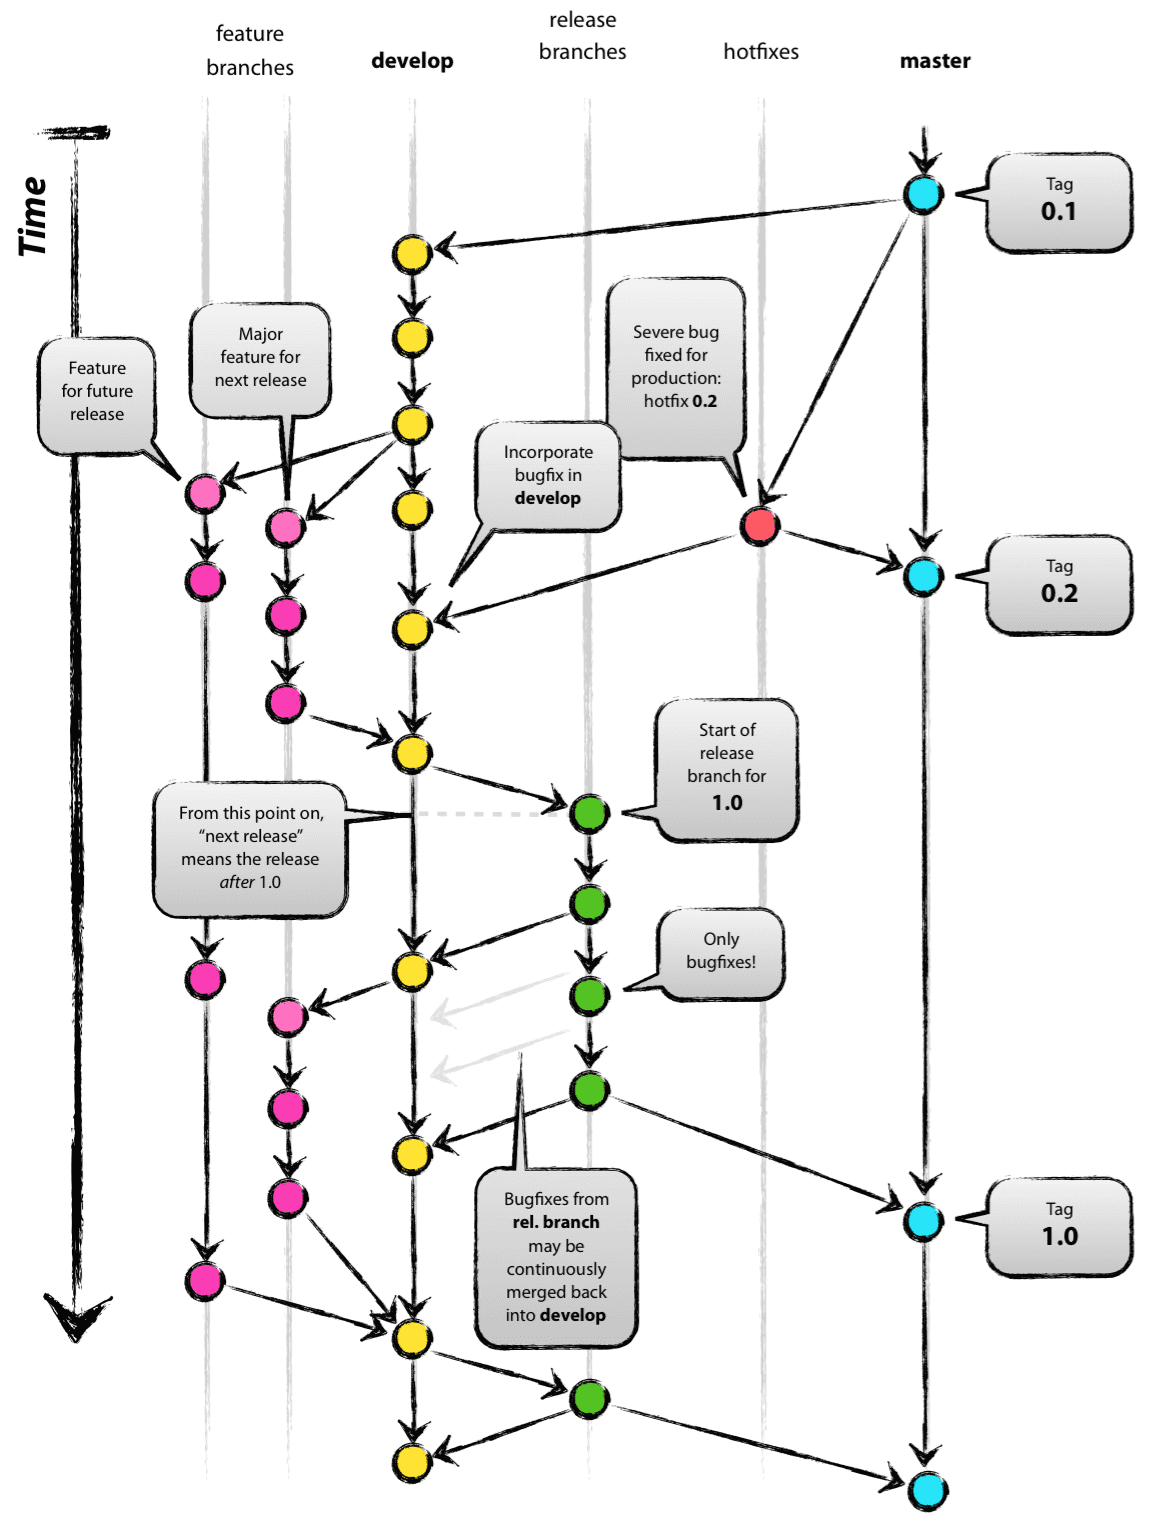
\includegraphics[width=\textwidth]{img/gitflow}
			\end{center}
		\end{column}
	\end{columns}
\end{frame}

\begin{frame}[fragile]{Developing new features}
	When a new feature must be added to the software, the team responsible for it should branch a \texttt{feature-myfeature} branch from \texttt{develop}.
	\begin{itemize}
		\item \texttt{git checkout -b feature-myfeature develop}
	\end{itemize}
	Once all the work has been done, the branch should get merged in \texttt{develop} and deleted. Even if fast-forward, the merge should be visible, to prevent history loss.
	\begin{itemize}
		\item \texttt{git checkout develop}
		\item \texttt{git merge --no-ff feature-myfeature}
		\item \texttt{git branch -d feature-myfeature}
	\end{itemize}
	In order to minimize the merging effort, it is a good practice to incorporate changes from \texttt{develop} from time to time (e.g. when another team completed another feature).
\end{frame}

\begin{frame}[fragile]{Releasing a new version}
	When the status of the \texttt{develop} branch is (besides the very last bits) the status of the next production release, a \texttt{release-version} should branch from \texttt{develop}.
	\begin{itemize}
		\item \texttt{git checkout -b release-version develop}
	\end{itemize}
	In this branch, only things like version number changes or last minute bug fixes should get incorporated. Once done, we merge the \texttt{release-version} branch back into \texttt{develop}...
	\begin{itemize}
		\item \texttt{git checkout develop}
		\item \texttt{git merge --no-ff release-version}
	\end{itemize}
	...and \texttt{master}. Plus, we tag master, so that we keep a reference to the exact repository status at release time. Then, we delete the \texttt{release-version} branch.
	\begin{itemize}
		\item \texttt{git checkout master}
		\item \texttt{git merge --no-ff release-version}
		\item \texttt{git tag -a version}
		\item \texttt{git branch -d release-version}
	\end{itemize}
\end{frame}

\begin{frame}[fragile]{Fix severe bugs affecting the mainline}
	You spot a bug in your current production branch. The fix must be delivered immediately.
	
	Start a new \texttt{hotfix-version} branch:
	\begin{itemize}
		\item \texttt{git checkout -b hotfix-version master}
	\end{itemize}
	Change the version number, fix the bug (also add a regression test). Once done, repeat the procedure already seen for a normal release.
	\begin{itemize}
		\item \texttt{git checkout develop}
		\item \texttt{git merge --no-ff hotfix-version}
		\item \texttt{git checkout master}
		\item \texttt{git merge --no-ff hotfix-version}
		\item \texttt{git tag -a version}
		\item \texttt{git branch -d hotfix-version}
	\end{itemize}
\end{frame}

\begin{frame}[fragile]{\texttt{git flow}}
	\begin{itemize}
		\item This workflow, first suggested by Vincent Driessen, got very popular.
		\item The command sequence is repetitive, and got automated
		\item A git extension (not part of the git distribution) is available:
		\begin{itemize}
			\item Introduces the \texttt{git flow} subcommand
			\item Starts and finishes feature, release, hotfix (and support)  branches
			\item Under the hood, it calls exactly the commands listed previously
		\end{itemize}
		\item My suggestion 
		\begin{itemize}
			\item \textit{learn} git flow as a development model
			\item Get acquainted with it using standard \texttt{git}
			\item When you are very confident that you know what the tool is doing with your repository, use \texttt{git flow}
			\item This is a good approach in general to new tools:
			\begin{itemize}
				\item understand the idea
				\item learn the basics
				\item understand what goes on under the hood
				\item use the advanced features productively
			\end{itemize}
		\end{itemize}
	\end{itemize}
\end{frame}

\subsection{with forks and pull requests}

\begin{frame}{A higher degree of control}
    It's not always a good idea to give writing permissions on your repository
    \begin{itemize}
        \item A student may push bad commits
        \item A wrong push on the wrong branch could have bad effects
        \item Your boss made a change but got tired of the push being refused and just uses \texttt{--force}
        \item You want fine grained control on the code that is being pushed
        \begin{itemize}
            \item e.g. perform code review
        \end{itemize}
    \end{itemize}
    How to enforce a higher degree of control, retaining the possibility to contribute?
\end{frame}

\begin{frame}{Forking}
    \begin{block}{fork}
        A hosted clone of a repository associated to a different user / team
    \end{block}
    \begin{itemize}
        \item Both Bitbucket and GitHub allow it
        \begin{itemize}
            \item Bitbucket allows multiple forks of the same repo by the same user
        \end{itemize}
        \item Every developer (or team) has his own fork where to work
        \item Makes changes freely
        \item Once complete, asks the maintainer of the original fork to \textit{pull} from its repository
        \begin{itemize}
            \item The maintainer of the original repository can choose whether or not to pull
            \item Possibly, provide a list of changes required for the pull to happen
        \end{itemize}
    \end{itemize}
\end{frame}

\begin{frame}{Working with pull requests}
    \begin{block}{pull request}
        An official request to incorporate changes from a branch of a fork to a branch of another fork.
    \end{block}
    \begin{itemize}
        \item Both Bitbucket and GitHub support the process
        \item A list of changes (commits) is pictured
        \item The merge is tested, and in case of conflict the pull request is suspended and can't be merged
        \begin{itemize}
            \item It is up to the requestor to provide mergeable code and fix conflicts
        \end{itemize}
        \item Code review can be performed by asking a number of changes and tracking the evolution
        \item Comments can be provided line by line
        \item Once the pull request satisfies the requirements, it can be merged and becomes part of the original repository
    \end{itemize}
\end{frame}


\section*{\refname}
%===============================================================================
\begin{frame}[allowframebreaks]
  \frametitle{\refname}
  \scriptsize
  \bibliographystyle{alpha}
  \bibliography{../bibliography}
\end{frame}
\section*{\refname}




\end{document}
